DKT numbers are means over 15 runs (3 seeds $\times$ 5 folds); numbers for simpleKT, AKT, QIKT and the pyKT DKT are means over 5 runs (5 folds, seed 42).
Differences are ``clear'', ``trend'' or ``not distinguishable'' as in Section~\ref{subsec:boot}; only clear differences are in bold in Tables~\ref{tab:decomp} and~\ref{tab:strata}.

\subsection{Main Results and Calibration}
\label{subsec:res-main}

% ===== TABLE 2 =====
\begin{table}[tbp]
  \caption{Main results on XES3G5M (mean over runs; $\pm$ is the sd over runs; DKT variants 15 runs, other models 5 runs). ACC uses a threshold of 0.5 and is not tested. Paired tests: Table~\ref{tab:decomp} (DKT) and Sect.~\ref{subsec:res-skt} (simpleKT). ``Ref.\ AUC'': value published for the pyKT model on XES3G5M.}
  \label{tab:main}
  \centering
  \scriptsize
  \setlength{\tabcolsep}{3pt}
  \resizebox{\textwidth}{!}{%
    \begin{tabular}{@{}lrllllrl@{}}
\toprule
Model & Runs & AUC & ACC & Brier & ECE & Params & Ref.\ AUC \\
\midrule
DKT & 15 & 0.7841 $\pm$ 0.0002 & 0.8172 & 0.1319 & 0.0111 $\pm$ 0.0015 & 588,465 & -- \\
DKT, leak-free selection & 15 & 0.7840 $\pm$ 0.0002 & 0.8172 & 0.1319 & 0.0111 $\pm$ 0.0015 & 588,465 & -- \\
DKT-ML & 15 & 0.7886 $\pm$ 0.0002 & 0.8189 & 0.1305 & 0.0056 $\pm$ 0.0022 & 674,965 & -- \\
DKT-ML-PQC & 15 & 0.7897 $\pm$ 0.0002 & 0.8192 & 0.1303 & 0.0047 $\pm$ 0.0014 & 674,965 & -- \\
DKT-PQC & 15 & 0.7891 $\pm$ 0.0002 & 0.8191 & 0.1304 & 0.0047 $\pm$ 0.0018 & 588,465 & -- \\
DKT-Fuse & 15 & 0.7894 $\pm$ 0.0001 & 0.8193 & 0.1303 & 0.0041 $\pm$ 0.0014 & 588,465 & -- \\
\midrule
DKT (pyKT) & 5 & 0.7834 $\pm$ 0.0001 & 0.8165 & 0.1322 & 0.0120 $\pm$ 0.0045 & 841,465 & 0.7852 \\
AKT (pyKT) & 5 & 0.8162 $\pm$ 0.0008 & 0.8261 & 0.1243 & 0.0172 $\pm$ 0.0014 & 6,824,518 & 0.8207 \\
QIKT (pyKT) & 5 & 0.8206 $\pm$ 0.0001 & 0.8294 & 0.1222 & 0.0076 $\pm$ 0.0074 & 13,290,684 & 0.8222 \\
\midrule
simpleKT (pyKT) & 5 & 0.8121 $\pm$ 0.0004 & 0.8235 & 0.1258 & 0.0191 $\pm$ 0.0017 & 3,754,497 & 0.8163 \\
simpleKT-PQC & 5 & 0.8164 $\pm$ 0.0004 & 0.8269 & 0.1238 & 0.0081 $\pm$ 0.0024 & 3,754,497 & -- \\
\bottomrule
\end{tabular}
%
  }
\end{table}

Table~\ref{tab:main} compares the models. The three PQC implementations of DKT reach an AUC of 0.7891--0.7897 against 0.7841 for standard DKT, and DKT-ML, which only removes the label from the context, lies in between (0.7886).
The ordering is the same for all three seeds, and the standard deviation over 15 runs (0.0001--0.0002) is about 25 times smaller than the gap between DKT-PQC and DKT.
DKT-PQC and DKT-Fuse add no parameters, so the gain does not come from model size; DKT-ML and DKT-ML-PQC add 86\,500 (+14.7\%) and are not better.
On simpleKT, the mask raises AUC by 0.0043 (0.0039--0.0050) and ACC from 0.8235 to 0.8269; AUC, Brier and ECE are clear in 5 of 5 runs.

PQC is not meant to close the gap between backbones: our best DKT variant is 0.022--0.027 below the pyKT simpleKT and AKT, while simpleKT-PQC is at the level of the pyKT AKT (0.8164 against 0.8162; no paired test) and 0.0042 below QIKT. Our pyKT runs are 0.0016--0.0045 below the published values (Table~\ref{tab:main}), so comparison with them is only indicative.

\paragraph{Calibration.}
The gain is not limited to ranking: ECE falls from 0.0111 to 0.0041--0.0047 and Brier from 0.1319 to 0.1303--0.1304.
The DKT variants with PQC are better calibrated than simpleKT (ECE 0.0191) and AKT (0.0172), although these have a higher AUC. On simpleKT the mask lowers ECE to 0.0081, close to QIKT (0.0076).

\subsection{Decomposition and Implementations}
\label{subsec:res-decomp}

% ===== TABLE 3 =====
\begin{table}[tbp]
  \caption{Paired bootstrap differences $b-a$ on DKT (AUC: mean [min; max] over 15 runs; CI: runs with CI above 0 / below 0; Brier and ECE: mean). Bold: clear difference.}
  \label{tab:decomp}
  \centering
  \scriptsize
  \setlength{\tabcolsep}{3pt}
  \resizebox{\textwidth}{!}{%
    \begin{tabular}{@{}l l c c c@{}}
\toprule
Comparison ($b-a$) & $\Delta$AUC [min; max] & CI & $\Delta$Brier & $\Delta$ECE \\
\midrule
DKT-ML $-$ DKT (i) & \textbf{+0.00448} [+0.00410; +0.00506] & 15 / 0 & \textbf{$-$0.00136} & \textbf{$-$0.00544} \\
DKT-ML-PQC $-$ DKT-ML (ii) & \textbf{+0.00109} [+0.00046; +0.00148] & 15 / 0 & \textbf{$-$0.00029} & $-$0.00092 \\
DKT-PQC $-$ DKT-ML-PQC (label) & \textbf{$-$0.00058} [$-$0.00121; $-$0.00005] & 0 / 10 & +0.00014 & $-$0.00005 \\
DKT-PQC $-$ DKT (total) & \textbf{+0.00499} [+0.00473; +0.00543] & 15 / 0 & \textbf{$-$0.00151} & \textbf{$-$0.00641} \\
\midrule
DKT-ML-PQC $-$ DKT & \textbf{+0.00557} [+0.00510; +0.00606] & 15 / 0 & \textbf{$-$0.00165} & \textbf{$-$0.00636} \\
DKT-Fuse $-$ DKT & \textbf{+0.00533} [+0.00483; +0.00568] & 15 / 0 & \textbf{$-$0.00161} & \textbf{$-$0.00696} \\
DKT-Fuse $-$ DKT-PQC & \textbf{+0.00034} [+0.00010; +0.00061] & 8 / 0 & \textbf{$-$0.00010} & $-$0.00055 \\
DKT-Fuse $-$ DKT-ML-PQC & $-$0.00024 [$-$0.00059; +0.00026] & 0 / 6 & +0.00004 & $-$0.00060 \\
\midrule
DKT-PQC $-$ DKT, leak-free selection & \textbf{+0.00506} [+0.00465; +0.00560] & 15 / 0 & \textbf{$-$0.00153} & \textbf{$-$0.00647} \\
DKT, leak-free selection $-$ DKT & $-$0.00007 [$-$0.00056; +0.00029] & 1 / 3 & +0.00002 & +0.00006 \\
\bottomrule
\end{tabular}
%
  }
\end{table}

Table~\ref{tab:decomp} separates the effect of the rule into the steps of Section~\ref{subsec:rule-def}.
Removing the label while keeping the sequential reading (condition (i), DKT $\to$ DKT-ML) adds 0.0045 AUC, and reading the state before the question (condition (ii), DKT-ML $\to$ DKT-ML-PQC) a further 0.0011; both are clear, with the interval excluding 0 in 15 of 15 runs.
Replacing MASK by the true label (DKT-ML-PQC $\to$ DKT-PQC) lowers AUC by 0.0006 (clear in sign, but small). The three steps add up exactly to the total $+0.0050$ in AUC, and likewise in Brier and ECE; most of the Brier and ECE gain comes from the first step.
The three implementations of the rule differ by at most 0.0006 AUC, about nine times less than the effect of the rule itself (DKT-Fuse is above DKT-PQC by 0.0003, interval excluding 0 in 8 of 15 runs; DKT-Fuse and DKT-ML-PQC cannot be distinguished).
We therefore do not rank them: what matters is that (i) and (ii) hold.
Finally, selecting the checkpoint of standard DKT with a leak-free criterion changes AUC by $-0.00007$ and the sign changes between runs (not distinguishable); against this variant DKT-PQC is still better by $+0.0051$ AUC, so the gain does not come from the way the checkpoint is chosen.

\subsection{Mechanism: Where the Gain Comes From}
\label{subsec:res-mech}

\paragraph{AUC by KC position.}
Figure~\ref{fig:kcpos} gives the KC-level AUC in multi-KC questions, for the first KC and for the second and later KCs.
Standard DKT is almost 0.10 AUC worse on the later KCs (0.7029) than on the first (0.8008; gap $-0.0978\pm0.0024$), and simpleKT and AKT show larger gaps ($-0.126$, $-0.135$).
This is what label copying predicts: under all-in-one evaluation the previous KC of the same question is not available, so the shortcut is useless exactly where it was learned.
The pyKT DKT shows the same drop ($-0.093$), so it does not come from our implementation.
DKT-ML, which still predicts KC $j$ after the earlier KCs of the question, is in between ($-0.048$).
With (ii) the gap is only about $-0.005$ (DKT variants) and $-0.0056$ (simpleKT-PQC), which we read as the baseline difficulty of later KCs.

\begin{figure}[tbp]
  \centering
  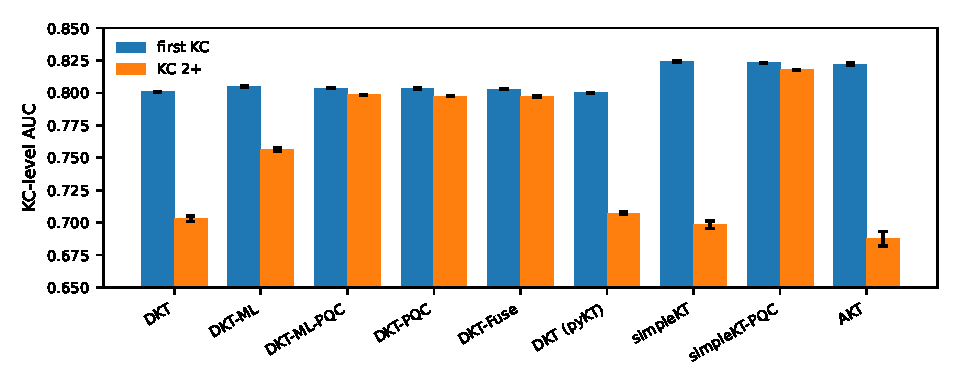
\includegraphics[width=\textwidth]{figures/fig2_kcpos.pdf}
  \caption{KC-level AUC in multi-KC questions, first KC against second and later KCs (mean over runs; error bars: sd over runs; DKT variants 15 runs, other models 5 runs). Diagnostic only, not used to rank models.}
  \label{fig:kcpos}
\end{figure}

\paragraph{AUC by question group.}
If leakage is the cause, the gain should be concentrated in multi-KC questions, and Table~\ref{tab:strata} shows that it is.
For DKT-PQC the AUC gain is $+0.0321$ on multi-KC targets (137\,481 questions) against $+0.0010$ on single-KC targets (961\,716); DKT-Fuse and DKT-ML-PQC behave the same way ($+0.0320$ and $+0.0328$ against $+0.0014$ and $+0.0016$).
For a fixed type of target the gain hardly depends on the previous question ($+0.0325$ and $+0.0314$ for multi-KC targets), so the target determines the gain, consistent with the leakage explanation.
On simpleKT the gain on multi-KC targets is similar ($+0.0242$, 5 of 5 folds), but on single-KC targets the mask is slightly worse ($-0.0027$, 5 of 5 folds); Sect.~\ref{subsec:res-skt} shows that this loss is concentrated in immediate repeats.

% ===== TABLE 4 (strata) =====
\begin{table}[tbp]
  \caption{Change in AUC by question group (target / previous question): DKT-PQC $-$ DKT (mean over 15 runs) and simpleKT-PQC $-$ simpleKT (mean over 5 runs). In parentheses: runs with a positive difference; then runs with CI above 0 / below 0. The last block (immediate repeats: the question ID equals that of the previous graded question) is given for simpleKT only, since DKT does not merge repeats (Sect.~\ref{subsec:int-simpleKT}). Bold: clear difference.}
  \label{tab:strata}
  \centering
  \scriptsize
  \setlength{\tabcolsep}{3pt}
  \resizebox{\textwidth}{!}{\begin{tabular}{@{}l r l@{}}
\toprule
Target / previous question & \#questions & DKT-PQC $-$ DKT (of 15) \\
\midrule
1 KC / all & 961\,716 & \textbf{+0.0010 (15; 15 / 0)} \\
multi-KC / all & 137\,481 & \textbf{+0.0321 (15; 15 / 0)} \\
\midrule
1 KC / 1 KC & 865\,139 & \textbf{+0.0011 (15; 15 / 0)} \\
1 KC / multi-KC & 93\,251 & +0.0006 (14; 2 / 0) \\
multi-KC / 1 KC & 93\,786 & \textbf{+0.0325 (15; 15 / 0)} \\
multi-KC / multi-KC & 43\,408 & \textbf{+0.0314 (15; 15 / 0)} \\
\midrule
1 KC / first graded question & 3\,326 & \textbf{$-$0.0067 (0; 0 / 9)} \\
multi-KC / first graded question & 287 & \textbf{+0.0452 (15; 12 / 0)} \\
all first graded questions & 3\,613 & +0.0001 (8; 0 / 0) \\
\bottomrule
\end{tabular}
}%
\end{table}

\subsection{Sanity Checks for Leakage}
\label{subsec:res-sanity}

Results of the checks of Section~\ref{subsec:sanity} (fold 0, seed 42):
\emph{Positive control:} flipping the label of a multi-KC question changes the prediction of its later KCs by up to 1.00 for standard DKT (flagged as leaking) and by 0 for DKT-PQC; the next question's prediction still changes in both, so the test is reliable.
\emph{Shuffled labels} (Table~\ref{tab:sanity}): with labels shuffled by question, only standard DKT learns from the shared label (best validation AUC 0.625); the four variants that satisfy (i) stay at 0.500--0.501. Test Brier separates them less cleanly (0.1631 for DKT and DKT-Fuse, 0.1625--0.1627 for the others), so we rely on validation AUC. With a global shuffle all variants fall to about 0.50, and all five fit 4 training sequences, so low scores under shuffling do not reflect an inability to learn.
\emph{Leak-free selection:} it gives the same test result as the default choice (AUC 0.7840 against 0.7841; Tables~\ref{tab:main} and~\ref{tab:decomp}), so the leakage is not an artifact of checkpoint selection.
These controls were run on DKT only; for simpleKT the evidence is the gap between first and later KCs and its removal by the mask (Figure~\ref{fig:kcpos}).

\subsection{First Graded Question of Each Student}
\label{subsec:res-first}

The gain is not uniform.
For the 3\,326 single-KC questions that are the first graded question of a student (0.3\% of the test questions), DKT-PQC is 0.0067 \emph{below} DKT: the difference is negative in all 15 runs and its interval excludes 0 in 9 (clear; Table~\ref{tab:strata}).
Over all 3\,613 first graded questions, including the 287 multi-KC ones (where DKT-PQC is 0.0452 \emph{above} DKT), the difference is $+0.0001$ and changes sign between runs, so this small group does not contradict the overall gain; we have not tested why standard DKT is better on it.
On simpleKT the mask is clearly better on the first graded questions as a whole ($+0.0087$, 5 of 5 folds; Table~\ref{tab:strata}): the gain on the 287 multi-KC ones ($+0.0399$) outweighs a small, not distinguishable difference on the single-KC ones ($-0.0012$).

\subsection{simpleKT-PQC versus simpleKT}
\label{subsec:res-skt}

Three criteria were fixed before the runs: (a) $\Delta$AUC $\ge 0.003$ and clear, (b) $\Delta$Brier $<0$ and clear, (c) a gap between later and first KCs within $\pm0.03$ in all five folds. All three hold. simpleKT-PQC raises AUC from 0.8121 to 0.8164 ($+0.0043$, from $+0.0039$ to $+0.0050$; CI excludes 0 in 5 of 5 folds), and lowers Brier by 0.0020 and ECE from 0.0191 to 0.0081, all clear (Table~\ref{tab:main}).
The gap between later and first KCs, $-0.1260\pm0.0032$ for simpleKT, becomes $-0.0056\pm0.0003$ (Figure~\ref{fig:kcpos}): the later KCs gain 0.1196 AUC and the first KC changes by $-0.0008$.
This is the pattern expected if the baseline copies the label of an earlier KC of its own question. Unlike DKT, simpleKT has no shuffle or intervention control, so the evidence agrees with label copying but does not isolate it.

\paragraph{Single-KC questions and immediate repeats.}
On single-KC questions the mask is slightly worse ($\Delta$AUC $=-0.0027$, from $-0.0033$ to $-0.0017$; negative in 5 of 5 folds, clear), while on multi-KC questions it is better ($+0.0242$; Table~\ref{tab:strata}).
The loss is concentrated in immediate repeats, i.e.\ a question attempted twice in a row. On the 9\,515 single-KC repeats ($0.99\%$ of the group) simpleKT-PQC is $0.1725$ AUC below simpleKT in all folds; on the 909 multi-KC repeats it is similar ($-0.1877$), so it does not depend on the number of KCs. Over all 10\,424 repeats (0.95\% of the test questions) $\Delta$AUC $=-0.1739$ and $\Delta$Brier $=+0.0616$ in 5 of 5 folds; $\Delta$ECE is $+0.0053$ with the same sign in all folds but a CI that includes 0 (trend).
On the other 99.05\% of the questions the gain is larger than overall ($\Delta$AUC $=+0.0062$ against $+0.0043$, 5 of 5 folds).
On single-KC questions that are not repeats the difference is $-0.0008$ (from $-0.0014$ to $+0.0001$); its sign changes between folds (not distinguishable by our rule), although the CI lies below 0 in 4 of 5 folds, so a small residual loss cannot be excluded.

A likely cause is our segment convention (Sect.~\ref{subsec:int-simpleKT}): consecutive attempts at the same question are merged, so the mask hides the attempt just before the one being predicted, which is legitimate history at test time and highly informative. In fold 0, 98.1\% of repeats are correct after a correct attempt, against 33.4\% after an incorrect one.
The rule does not require this merge, but we have not isolated its effect, and group AUCs are not additive.

\begin{table}[tbp]
  \caption{Sanity checks on fold 0 (seed 42), DKT variants. Intervention test: \texttt{inside} / \texttt{after}. Brier of a constant predictor: about 0.1626.}
  \label{tab:sanity}
  \centering
  \scriptsize
  \setlength{\tabcolsep}{3pt}
  \resizebox{\textwidth}{!}{%
    \begin{tabular}{@{}l c c c c c@{}}
  \toprule
  Check & DKT & DKT-PQC & DKT-ML & DKT-ML-PQC & DKT-Fuse \\
  \midrule
  Intervention, inside / after           & 1.00 / 0.80 (leaks) & 0 / 0.76 (pass) & -- & -- & -- \\
  Overfit 4 sequences, loss after 300 steps & 0.0013 & 0.0013 & 0.0013 & 0.0013 & 0.0014 \\
  Shuffle by question: best val.\ AUC    & 0.6250 & 0.5005 & 0.5004 & 0.5002 & 0.5008 \\
  Shuffle by question: test Brier        & 0.1631 & 0.1625 & 0.1626 & 0.1627 & 0.1631 \\
  Global shuffle: best val.\ AUC         & 0.5010 & 0.5007 & 0.5011 & 0.5012 & 0.5009 \\
  Global shuffle: test Brier             & 0.1630 & 0.1630 & 0.1627 & 0.1628 & 0.1629 \\
  \bottomrule
\end{tabular}%%
  }
\end{table}